\subsection{\textbf{Etat de l'art de la détection des têtes}}

La détection des têtes est un sujet fondamental en vision par ordinateur, notamment pour des applications variées telles que la surveillance de foules, et les interactions homme-machine. Ce problème est souvent abordé avec des techniques similaires à la détection d'objets, en particulier les approches basées sur l'apprentissage profond.

\subsubsection{\textbf{Modèles basés sur les Réseaux de Neurones Convolutifs (CNNs)}}
Les CNNs sont les architectures les plus populaires pour la détection d'objets grâce à leur capacité à extraire des caractéristiques discriminantes \cite{lecun1998gradient}. Les architectures telles que Faster R-CNN \cite{ren2015faster}, SSD \cite{liu2016ssd} et RetinaNet \cite{lin2017focal} ont été adaptées pour la détection des têtes grâce à leur capacité à gérer différentes tailles.

\subsubsection{\textbf{Modèles basés sur YOLO}}
YOLO (You Only Look Once) est une approche de détection d'objets qui allie vitesse et précision \cite{redmon2016you}. Depuis YOLOv1 jusqu'à YOLOv11, les améliorations successives ont permis d'obtenir des performances toujours plus optimales en termes de précision et d'efficacité \cite{bochkovskiy2020yolov4, jocher2023ultralytics}. YOLO est particulièrement adapté à la détection en temps réel, ce qui le rend pertinent pour des applications de surveillance de personnes \cite{ge2019efficient, lian2021locating}. 
Récemment, YOLOv12 \cite{tian2025yolov12attentioncentricrealtimeobject} a introduit une architecture centrée sur les mécanismes d'attention tout en maintenant une vitesse d'inférence comparable aux modèles CNN classiques. Cette approche permet d'améliorer la qualité de la détection tout en conservant des performances adaptées aux besoins des applications en temps réel.


\subsection{Présentation des datasets}

Dans notre étude, nous recherchons des données contenant un grand nombre de personnes, car notre objectif est de nous intéresser spécifiquement aux foules denses. Pour faciliter les premières expérimentations, nous avons cependant commencé avec une densité plus faible. On portera une attention particulière à l'annotation des têtes, qu'on souhaite utiliser par la suite pour affiner notre estimation de la profondeur, la tête humaine ayant une taille relativement constante.

À cette fin, nous avons sélectionné le dataset CrowdHuman \cite{shao2018crowdhuman}, qui contient des images de très bonnes qualités à faible densité et très bien annotées. Ensuite, nous avons utilisé JHU-Crowd++ \cite{sindagi2020jhu-crowd++}, avec des images de moins bonnes qualités, aux annotations plus sommaires et mal définies au niveau des têtes.
Par ailleurs, nous avons identifié deux autres datasets similaires que nous n'avons pas exploités dans ce projet : NWPU-Crowd \cite{gao2020nwpu}, et UCF-QNRF \cite{idress2018ucfqnrf} contenant 1 535 images affichant une densité moyenne de 815 personnes par image.


\begin{table}[h]
    \centering
    \scriptsize
    \begin{tabularx}{\linewidth}{l>{\raggedright\arraybackslash}Xc}
            \toprule
            \textbf{Dataset} & \textbf{Nombre d'images} & \textbf{Personnes par image (moyenne)} \\
            \midrule
            CrowdHuman \cite{shao2018crowdhuman} & 15 000 & 22.64 \\
            JHU-Crowd++ \cite{sindagi2020jhu-crowd++} & 4 372 & 346 \\
            NWPU-Crowd \cite{gao2020nwpu} & 5 109 & 418 \\
            UCF-QNRF \cite{idress2018ucfqnrf} & 1 535 & 815 \\
            \bottomrule
        \end{tabularx}
    \caption{Tableau récapitulatif des datasets considérés.}
    \label{tab:datasets}
\end{table}


\subsection{Finetuning des modèles YOLO}

Pour la détection des têtes, nous avons choisi d'affiner des modèles de différentes tailles, YOLOv11 et YOLOv12, pré-entraînés sur le dataset COCO \cite{lin2015microsoftcococommonobjects}. La bibliothèque développée par Ultralytics, qui contient ces modèles YOLO, intègre ses propres méthodes de fine-tuning adaptées.
Dans un premier temps, nous avons utilisé le dataset CrowdHuman, puis nous avons essayé d'adapter notre modèle à une plus grande échelle avec JHU-Crowd++, en modifiant les annotations pour ne conserver que les têtes, conformément au format attendu par YOLO. Nous avons également enrichi l'entraînement avec des données synthétiques générées par le module Ultralytics appelé \textit{Mosaic}, qui combine plusieurs images pour créer une nouvelle image d'entraînement, améliorant ainsi la robustesse du modèle.
L'optimiseur Adam a été utilisé pour l'entraînement. Nous avons exploité un GPU A100, fourni par CentraleSupélec, avec 9.5GB de mémoire disponible. La taille du batch et celle des images ont été ajustées pour ne pas dépasser cette limite, selon la taille du modèle (en pratique, les versions \textit{nano} et \textit{large} ont été entraînées).
Notre modèle n'a qu'une seule classe, celle des têtes, contrairement aux modèles pré-entraînés YOLO qui comprennent plusieurs classes. Les performances sont évaluées sur le dataset de validation en utilisant la \textit{mean Average Precision} (mAP) et le \textit{F1-score} comme principales métriques. Les résultats obtenus sont ensuite analysés pour comprendre les limites du modèle et identifier des pistes d'amélioration.
Le dataset de test a été réalisé en prenant 20\% des données de chaque dataset, et en les mélangeant pour obtenir un dataset de test équilibré, et qui généralise au mieux. Les résultats sont présentés dans la section suivante. De plus, nous gardons les poids du modèle qui a le meilleur mAP sur le dataset de validation, pour simuler un early stopping.

\subsection{Résultats quantitatifs}

Sur le dataset CrowdHuman, nous avons essayé plusieurs modèles YOLO de différentes tailles, pour comparer leurs performances. Les résultats obtenus sont présentés dans le tableau \ref{tab:heads-detection}. Nous avons trouvé les meilleurs résultats avec le modèle large de YOLOv11, mais ce n'était pas significativement meilleur que les autres modèles. Nous avons donc décidé de sélectionner avec le modèle nano de YOLOv11 pour la suite de nos expérimentations, car il est plus rapide et moins gourmand en ressources.

\begin{table}[h]
    \centering
    \scriptsize
    \begin{tabularx}{\linewidth}{>{\raggedright\arraybackslash}Xcc}
        \toprule
        \textbf{Modèle} & \textbf{mAP} & \textbf{F1-score} \\
        \midrule
        YOLOv11 nano & 0.67 & 0.69 \\
        YOLOv11 large & 0.70 & 0.72 \\
        YOLOv12 nano & 0.66 & 0.68 \\
        YOLOv12 large & 0.67 & 0.69 \\
        \bottomrule
    \end{tabularx}
    \caption{Résultats quantitatifs de la détection des têtes selon la taille du modèle.}
    \label{tab:heads-detection-taille}
\end{table}

Les résultats obtenus sur le dataset CrowdHuman sont très satisfaisants, avec un mAP de 0.65 et un f1-score de 0.68. Cependant, le modèle n'arrive pas à apprendre sur le dataset JHU-Crowd++, avec un mAP de 0.1 et un f1-score de 0.14. Ces résultats montrent que le modèle peine à généraliser à des densités plus élevées, dû sûrement à la mauvaise qualité du dataset, et au fait que, à une certaine densité, les têtes ne sont pas très visibles. On a donc essayé une approche alternative pour augmenter la densité Les résultats: nous avons fine-tuner une seconde fois, avec un learning rate plus bas, sur les images avec moins de 150 personnes et ne contenant pas de têtes floues de JHU-crowd++, et nous avons réussi à augmenter grâce à cela les résultats de notre modèle.

\begin{table}[h]
    \centering
    \scriptsize
    \begin{tabularx}{\linewidth}{>{\raggedright\arraybackslash}Xcc}
        \toprule
        \textbf{Dataset} & \textbf{mAP} & \textbf{F1-score} \\
        \midrule
        CrowdHuman & 0.65 & 0.68 \\
        JHU-Crowd++ & 0.1 & 0.14 \\
        CrowdHuman + JHU-Crowd++ & 0.66 & 0.7 \\
        \bottomrule
    \end{tabularx}
    \caption{Résultats quantitatifs de la détection des têtes selon le dataset.}
    \label{tab:heads-detection}
\end{table}

\subsection{Résultats qualitatifs}

Comme on peut l'observer sur l'exemple Figure \ref{fig:heads-detection}, la détection des têtes est plutôt bonne, lorsque l'on est dans les champs proches et/ou que l'on voit bien la tête.

Cependant le modèle atteint ses limites lorsqu'il y a trop de têtes sur l'image, ou que celles-ci sont partiellement cachées ou en mauvaise résolution (car trop loin).

\begin{figure}[h!]
    \centering
    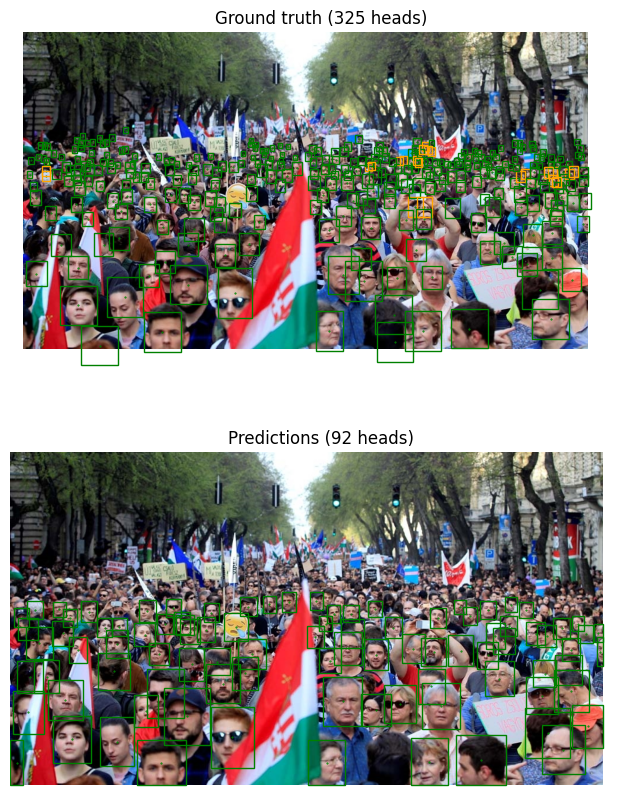
\includegraphics[width=0.45\textwidth]{images/heads_detection.png}
    \caption{Résultats de la détection des têtes.}
    \label{fig:heads-detection}
\end{figure}

De même, on peut comparer notre modèle finetuné au modèle sans finetuning qui contient une classe "personne" et non "tête". On peut voir sur la Figure \ref{fig:heads-detection-compare} que notre modèle finetuné est bien plus précis que le modèle sans finetuning, qui détecte moins d'1/3 des personnes dans une foule peu dense.

\begin{figure}[h]
    \centering
    \begin{minipage}{0.45\textwidth}
        \centering
        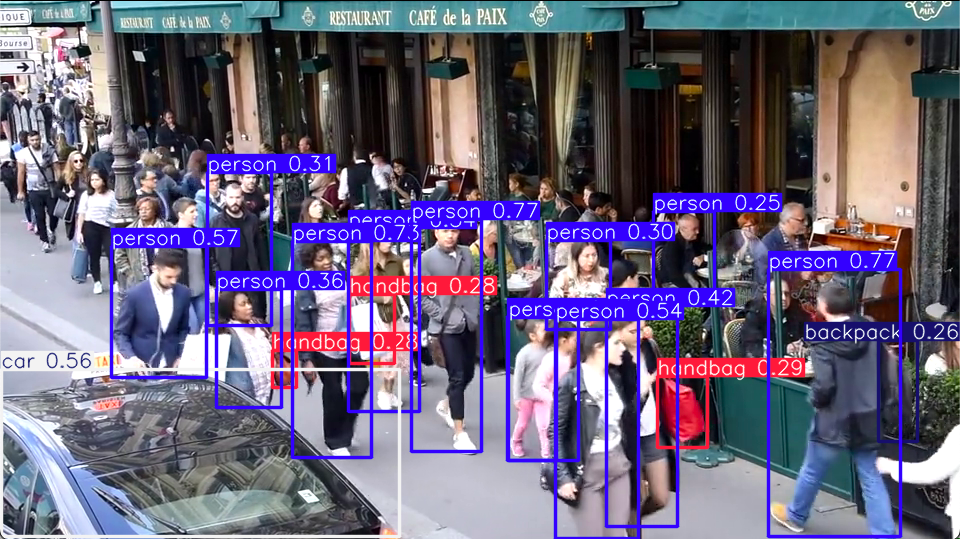
\includegraphics[width=\textwidth]{images/YOLO.png}
        \caption{Modèle YOLO non-finetuné (13 personnes détectées)}
    \end{minipage}
    \hfill
    \begin{minipage}{0.45\textwidth}
        \centering
        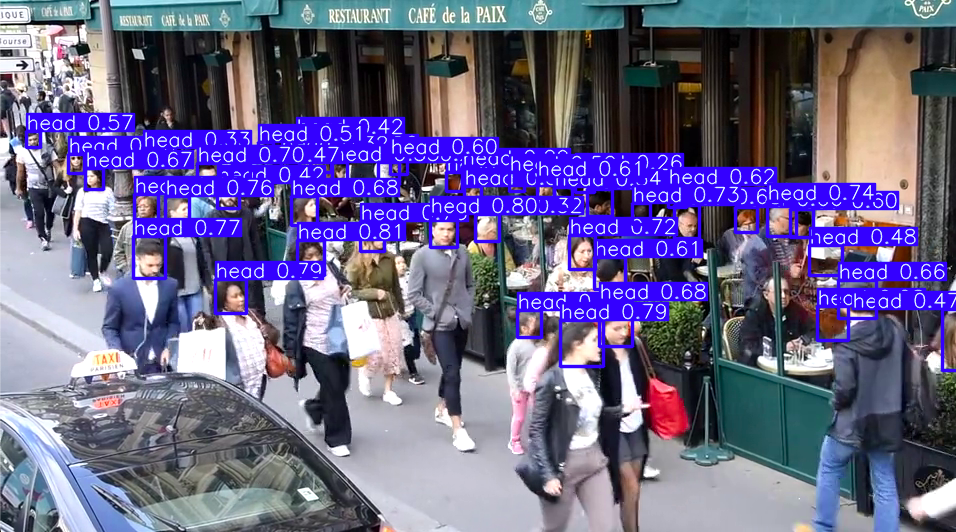
\includegraphics[width=\textwidth]{images/YOLOfinetuned.png}
        \caption{Modèle YOLO finetuné sur la détection de têtes (36 personnes détectées)}
    \end{minipage}
    \caption{Comparaison de la détection de têtes entre un modèle YOLO non-finetuné et finetuné}
    \label{fig:heads-detection-compare}
\end{figure}
